\documentclass{article}

\PassOptionsToPackage{numbers, compress}{natbib}
\usepackage[sglblindworkshop, final]{neurips_2026}
\workshoptitle{Predictive AI Evaluation Competition}

\usepackage[utf8]{inputenc}
\usepackage[T1]{fontenc}
\usepackage{hyperref}
\usepackage{url}
\usepackage{booktabs}
\usepackage{amsmath}
\usepackage{amssymb}
\usepackage{amsfonts}
\usepackage{nicefrac}
\usepackage{microtype}
\usepackage{xcolor}
\usepackage{graphicx}
\usepackage{enumitem}
\usepackage{algorithm}
\usepackage{algpseudocode}

\makeatletter
\renewcommand{\paragraph}{\@startsection{paragraph}{4}{\z@}{0.1ex \@plus 0.1ex}{-1em}{\normalsize\bf}}
\makeatother

\algblockdefx[Phase]{Phase}{EndPhase}[1]{\textbf{#1}}{}
\algnotext{EndPhase}
\algrenewcommand\algorithmicrequire{\textbf{Input:}}

\usepackage{colortbl}
\usepackage{pgf}
\definecolor{better}{HTML}{2A78D6}
\definecolor{worse}{HTML}{E34948}
\definecolor{neutral}{HTML}{8C8B86}
% value shading in tables (tools/shade_tables.py): \shd{value}{center}{span}{sign}, \shs{colour}{value}{lo}{hi},
% \shq{colour}{value}{hi}; \shmax is the strongest colour share in percent
\newcommand{\shmax}{35}
\newcommand{\shd}[4]{\pgfmathsetmacro{\shx}{(#4)*((#2)-(#1))/(#3)}\pgfmathsetmacro{\shp}{min(1,abs(\shx))*\shmax}%
  \pgfmathparse{\shx>0 ? 1 : 0}\ifnum\pgfmathresult=1\relax\edef\shc{\noexpand\cellcolor{better!\shp}}%
  \else\edef\shc{\noexpand\cellcolor{worse!\shp}}\fi\shc}
\newcommand{\shs}[4]{\pgfmathsetmacro{\shp}{max(0,min(1,((#2)-(#3))/((#4)-(#3))))*\shmax}%
  \edef\shc{\noexpand\cellcolor{#1!\shp}}\shc}
\newcommand{\shq}[3]{\pgfmathsetmacro{\shp}{sqrt(max(0,min(1,(#2)/(#3))))*\shmax}%
  \edef\shc{\noexpand\cellcolor{#1!\shp}}\shc}

\setcounter{topnumber}{1}
\renewcommand{\topfraction}{0.85}

\newcommand{\todo}[1]{\textcolor{red}{[#1]}}
\newcommand{\logit}{\operatorname{logit}}
\newcommand{\alc}{\mathrm{ALC}}

\title{A Language-Model Prior for Cold-Start Prediction\\of AI Evaluation Outcomes}

\author{%
  Minseung Lee \\
  \texttt{leemiinseung@gmail.com} \\
}

\begin{document}

\maketitle

\begin{abstract}
Deploying an AI system requires knowing how it will perform on its tasks, yet running every candidate on all of them is rarely affordable. Predictive evaluation estimates whether a system will succeed on an item it has not been run on, as item response theory does for test-takers. Its hardest case is a new benchmark with few or no outcomes, the benchmark-level cold start posed by the Predictive AI Evaluation Competition. There, in our tests, models fit to other benchmarks' outcomes barely beat a counting baseline. We combine a language-model prior with a hierarchical logistic model. The language model, the \emph{forecaster}, states a success probability from the system's description and the item, and the hierarchical model corrects it per benchmark and system as outcomes arrive. On held-out evaluations shaped like the competition, Claude Opus 5.5 cuts the area under the Brier learning curve from 0.214 for that baseline to 0.169, mostly through the forecast alone. Eight other forecasters gain half to four fifths as much and, once recalibrated, rank items and judge benchmark difficulty less well. On problems newer than the forecaster's training cutoff, the method only ties the baseline.
\end{abstract}
\suppressfloats[t]

\section{Introduction}

Anyone deploying an AI system needs to know how it will perform on the tasks it will face, and running every candidate system on all of them is rarely affordable \cite{zhou2026adele, paiec2026}. Item response theory meets the same need for human tests by predicting a test-taker's answers to items not yet given \cite{lord1980irt}, and predictive evaluation asks the same of AI systems. The Predictive AI Evaluation Competition poses its hardest case, a benchmark-level cold start \cite{paiec2026}. A predictor estimates the probability that an AI system answers an item correctly, without running the system, on benchmarks it has never seen and with at most 31 revealed outcomes per system--benchmark pair, and the score weights the first few outcomes most.

\begin{figure}[t]
  \centering
  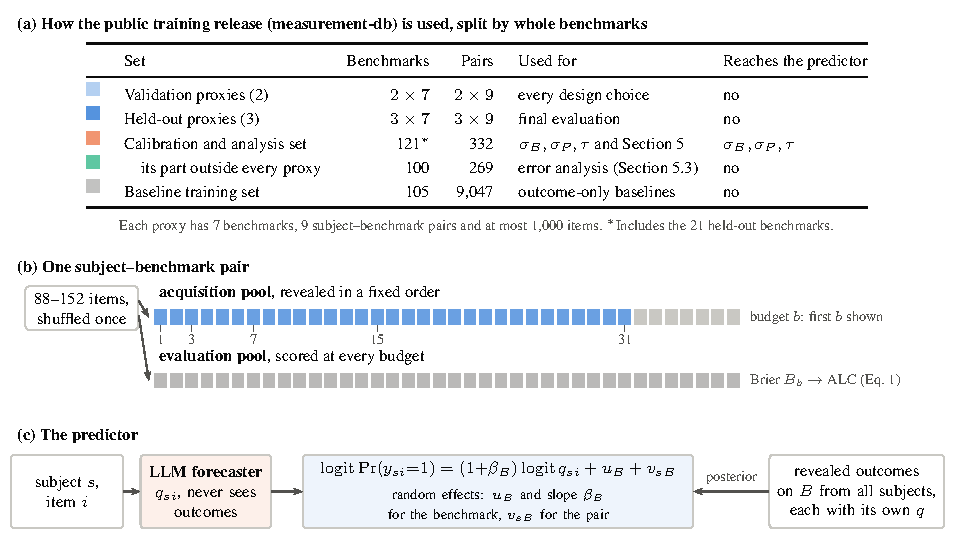
\includegraphics[width=\linewidth]{figures/fig_data.pdf}
  \vspace{-9pt}
  \caption{Data and method. (a) How each part of measurement-db is used. (b) Within a pair, half the items are revealed in a fixed order and half are scored at every budget. (c) A language model states the forecast $q_{si}$ without seeing outcomes, and revealed outcomes update the random effects.}
  \label{fig:data}
\end{figure}

Outcome data from other benchmarks do not solve it. An item response model \cite{lord1980irt} with subject attributes, model identity and item features, fit to 9{,}047 public pairs, scores within 0.003 of a Beta-binomial counting baseline, which shrinks each pair's success rate toward that of the other subjects on the benchmark, on five proxy evaluations (copies of the test built from public data, Section~\ref{sec:task}), and before any outcome is revealed both score close to the 0.250 of answering 0.5 (Table~\ref{tab:main}, Figure~\ref{fig:main}a). What separates an easy benchmark from a hard one is written in the items and in the system's description, which such models do not read.

We read the items and the system's description with a language model, the \emph{forecaster} (Figure~\ref{fig:data}c). It states a success probability, the \emph{forecast}, once per subject and item and never sees an outcome. The forecast enters a hierarchical logistic model as an offset, and random effects for the benchmark and for the subject on it, including a benchmark-specific slope on the forecast, absorb the revealed outcomes (Section~\ref{sec:method}). Our findings are the following.
\begin{itemize}
  \item \textbf{The forecast carries most of the gain.} With Claude Opus 5.5 as the forecaster, ALC falls by 0.045 against the Beta-binomial baseline on three held-out proxies, and the forecast alone, which never sees an outcome, captures 0.042 of it (Section~\ref{sec:results}).
  \item \textbf{Weaker forecasters gain less.} Eight other models gain half to four fifths as much once each has its own fitted constants (Section~\ref{sec:ladder}).
  \item \textbf{Opus leads in ranking items and in judging each benchmark's overall difficulty.} The ranking gap follows general capability closely and the benchmark gap only loosely (Section~\ref{sec:lead}).
  \item \textbf{Two questions stay open.} After the forecaster's training cutoff the method only matches the baseline (Section~\ref{sec:cutoff}), and whether recognizing a benchmark helps is unresolved (Section~\ref{sec:memory}).
\end{itemize}

\section{Task and evaluation data}
\label{sec:task}

Predictions are scored per subject--benchmark pair as more of the pair's outcomes are revealed, and we evaluate on public data arranged like the hidden test.

\begin{figure}[t]
  \centering
  \begin{minipage}[t]{0.6\linewidth}
    \vspace{0pt}
    {\footnotesize (a) tau2-bench, customer-service agent tasks}\par\vspace{2pt}
    {\scriptsize Subjects $s$: OpenAI GPT-4.1 mini and o4-mini, both released April 2025, in the \mbox{tau2-bench} harness. The predictor sees the benchmark only as an anonymous id.}\par\vspace{3pt}
    \scriptsize
    \setlength{\tabcolsep}{2.0pt}
    \begin{tabular}{@{}lccccc@{}}
    \toprule
    & & \multicolumn{3}{c}{Prediction at budget} & \\
    \cmidrule(lr){3-5}
    Item: domain, request & Forecast & 1 & 7 & 31 & Outcome \\
    \midrule
    \multicolumn{6}{@{}l}{\emph{GPT-4.1 mini, five of its 59 scored items}} \\
    airline: ``You want to cancel\ldots'' & \shs{better}{0.75}{0}{1} 0.75 & \shs{better}{0.79}{0}{1} 0.79 & \shs{better}{0.93}{0}{1} 0.93 & \shs{better}{0.93}{0}{1} 0.93 & 4 of 4 \\
    retail: ``You want to return the\ldots'' & \shs{better}{0.35}{0}{1} 0.35 & \shs{better}{0.51}{0}{1} 0.51 & \shs{better}{0.80}{0}{1} 0.80 & \shs{better}{0.78}{0}{1} 0.78 & 4 of 4 \\
    airline: ``You want to first cancel\ldots'' & \shs{better}{0.25}{0}{1} 0.25 & \shs{better}{0.41}{0}{1} 0.41 & \shs{better}{0.73}{0}{1} 0.73 & \shs{better}{0.71}{0}{1} 0.71 & 0 of 4 \\
    telecom: ``You mobile data is not\ldots'' & \shs{better}{0.12}{0}{1} 0.12 & \shs{better}{0.26}{0}{1} 0.26 & \shs{better}{0.57}{0}{1} 0.57 & \shs{better}{0.54}{0}{1} 0.54 & 2 of 4 \\
    telecom: ``You are unable to send\ldots'' & \shs{better}{0.05}{0}{1} 0.05 & \shs{better}{0.15}{0}{1} 0.15 & \shs{better}{0.38}{0}{1} 0.38 & \shs{better}{0.35}{0}{1} 0.35 & 0 of 4 \\
    Beta-binomial baseline, every item & & \shs{better}{0.53}{0}{1} 0.53 & \shs{better}{0.79}{0}{1} 0.79 & \shs{better}{0.70}{0}{1} 0.70 & \\
    \midrule
    \multicolumn{6}{@{}l}{\emph{Update from both subjects' revealed outcomes}} \\
    Successes revealed, GPT-4.1 mini & & 0 of 1 & 6 of 7 & 22 of 31 & \\
    Successes revealed, o4-mini & & 1 of 1 & 5 of 7 & 21 of 31 & \\
    $u_B$ (benchmark) & $0$ & $+0.63$ & $+1.78$ & $+1.59$ & \\
    $\beta_B$ (slope) & $0$ & $-0.05$ & $-0.13$ & $-0.15$ & \\
    $v_{sB}$, GPT-4.1 mini & $0$ & $-0.02$ & $+0.24$ & $+0.26$ & \\
    $v_{sB}$, o4-mini & $0$ & $+0.13$ & $+0.08$ & $+0.03$ & \\
    \bottomrule
\end{tabular}

  \end{minipage}\hfill
  \begin{minipage}[t]{0.375\linewidth}
    \vspace{0pt}
    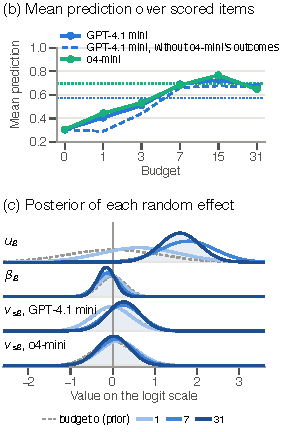
\includegraphics[width=\linewidth]{figures/fig_worked.pdf}
  \end{minipage}
  \caption{Revealed outcomes correct a forecast that ranks items fairly well but sets their level too low. One held-out benchmark, tau2-bench, with two subjects, chosen to show each random effect (Section~\ref{sec:infer}). (a) Five GPT-4.1 mini items, evenly spaced in forecast rank and shown by domain and the first words of the customer's request. Outcome counts successes in the four attempts recorded per task. (b) Mean prediction over each subject's scored items, with dotted lines at the success rates. The dashed line leaves out o4-mini's outcomes. (c) Laplace posterior of each random effect at budgets 0 (the prior), 1, 7 and 31, each row scaled to its own height.}
  \label{fig:worked}
\end{figure}

\paragraph{Subjects, items and responses.} A subject $s$ is an AI system with a fixed model, harness and reasoning effort. An item $i$ carries its text, features, interactors (other tools or agents involved) and an anonymous benchmark id. A response $y_{si} \in \{0,1\}$ records one attempt, so an item may have several responses.

\paragraph{Budgets and score.} Each pair is scored at six label budgets, evenly spaced on a log scale so that the first few revealed outcomes count most. The platform splits the pair's items into an acquisition pool, whose candidates arrive in a fixed random order, and an evaluation pool that is scored at every budget (Figure~\ref{fig:data}b). At label budget $b$ the outcomes of the first $b$ candidates are revealed. A submission may supply a rule that skips candidates. Ours keeps the fixed order, and so does every table except the acquisition experiment of Section~\ref{sec:labels}. The score is the area under the learning curve (ALC) of Brier against budget. With $B_b$ the Brier score at budget $b$, averaged first within and then across pairs,
\begin{equation}
  \alc = 0.1\,B_0 + 0.2\,B_1 + 0.2\,B_3 + 0.2\,B_7 + 0.2\,B_{15} + 0.1\,B_{31}.
  \label{eq:alc}
\end{equation}

\paragraph{Hidden test.} The test benchmarks are hidden and disjoint from the public training release, measurement-db \cite{measurementdb2026}. During the competition the platform scores submissions on formative samples, sets of hidden pairs from seven benchmarks.

\paragraph{Proxy evaluations.} Five proxy evaluations built from measurement-db stand in for the hidden test, each with the shape of a formative sample, seven benchmarks, nine pairs and at most 1{,}000 items (Figure~\ref{fig:data}a, Appendix~\ref{app:proxies}). Two validation proxies (18 pairs) served every design choice. Three held-out proxies (27 pairs), drawn later without overlap, were first evaluated after the forecaster, the prompt, $\sigma_B$ and $\sigma_P$ were fixed. We added the benchmark slope $\beta_B$ (Section~\ref{sec:model}) after seeing their results and those on MathArena (Section~\ref{sec:cutoff}), and their benchmarks also appear in the calibration set below (Section~\ref{sec:limits}).

\paragraph{Calibration set.} A calibration and analysis set of 121 measurement-db benchmarks outside the validation proxies (332 pairs, seven items from each) fixes the constants of our model and serves the analyses of Section~\ref{sec:analysis}.


\section{Method}
\label{sec:method}

Our predictor combines a forecast that never sees an outcome with a hierarchical model that the revealed outcomes update. Figure~\ref{fig:worked} follows it through one benchmark, and Algorithm~\ref{alg:predict} in Appendix~\ref{app:repro} gives the procedure.

\begin{figure}[t]
  \centering
  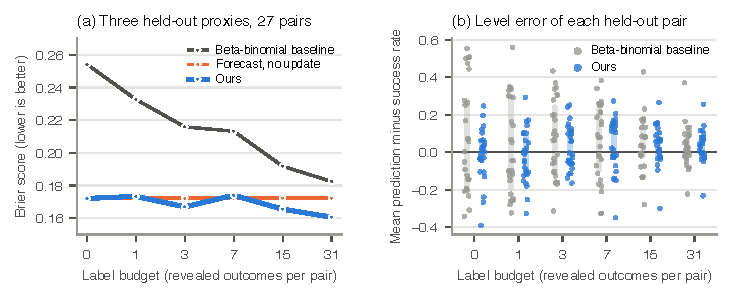
\includegraphics[width=\linewidth]{figures/fig_main.pdf}
  \vspace{-9pt}
  \caption{Our method stays below the Beta-binomial baseline at every budget, and most of the gap is there before any outcome is revealed. Three held-out proxies, 27 pairs. (a) Brier by budget. (b) Each pair's mean prediction minus its success rate, with bars spanning the middle half of the 27 pairs.}
  \label{fig:main}
\end{figure}


\subsection{Forecast}

The forecaster, Claude Opus 5.5 at low effort, returns $q_{si} \in [0,1]$ from the subject's fields and the item's fields alone (prompt in Appendix~\ref{app:prompts}). Higher effort did not help (Appendix~\ref{app:ablations}).

\subsection{Model}
\label{sec:model}

Outcomes on benchmark $B$ follow the logistic mixed model
\begin{equation}
  \logit \Pr(y_{si} = 1) = (1 + \beta_B) \logit q_{si} + u_B + v_{sB},
  \label{eq:model}
\end{equation}
in which the forecast's logit is an offset with its coefficient centred at 1, and three random effects correct it:
\begin{itemize}[leftmargin=1.5em, itemsep=1pt, topsep=3pt]
  \item $u_B \sim \mathcal{N}(0, \sigma_B^2)$, a benchmark intercept, the forecast's overall error on $B$, shared by all subjects,
  \item $\beta_B \sim \mathcal{N}(0, \tau^2)$, a benchmark slope, how far the forecast's differences between items are trusted on $B$,
  \item $v_{sB} \sim \mathcal{N}(0, \sigma_P^2)$, a subject-by-benchmark intercept, the error specific to subject $s$ on $B$.
\end{itemize}
The offset follows explanatory item response models \cite{deboeck2004explanatory}, $\beta_B$ plays the role of an item discrimination, and $v_{sB}$ that of a person-by-testlet effect \cite{bradlow1999testlet}.

\paragraph{Fitting the constants.} All three standard deviations come from the calibration set.
\begin{itemize}[leftmargin=1.5em, itemsep=1pt, topsep=3pt]
  \item $\sigma_B = 1.09$ and $\sigma_P = 0.46$ come from the method of moments. Each pair's forecast error, $\logit(\text{mean forecast}) - \logit(\text{success rate})$, is split into a between-benchmark and a within-benchmark variance, after removing the sampling noise of seven-item means.
  \item $\tau = 0.30$ maximizes the Laplace-approximated marginal likelihood of the calibration set with $\sigma_B$ and $\sigma_P$ fixed, each item counted once with its success rate as a fractional outcome.
\end{itemize}

\subsection{Inference and prediction}
\label{sec:infer}

\paragraph{Update.} Revealed outcomes from every subject on $B$ update the random effects (Algorithm~\ref{alg:predict}, line~\ref{alg:update}, with details in Appendix~\ref{app:repro}). Each outcome enters Equation~\eqref{eq:model} with its own forecast as offset, so a success on an item the forecaster already rated easy moves them less than a success on an item it rated hard.

\paragraph{Prediction.} The prediction averages over the posterior with the probit approximation \cite{mackay1992evidence},
\begin{equation}
  \hat p_{si} = \operatorname{sigmoid}\!\left( \frac{(1 + \mu_{\beta}) \logit q_{si} + \mu_{u} + \mu_{v}}{\sqrt{1 + \pi\sigma^2/8}} \right),
  \label{eq:pred}
\end{equation}
where $\mu_u$, $\mu_\beta$ and $\mu_v$ are the posterior modes of $u_B$, $\beta_B$ and $v_{sB}$, and $\sigma^2$ is the posterior variance of $u_B + \beta_B \logit q_{si} + v_{sB}$.

\paragraph{What the update keeps.} The forecaster's differences between items survive the update unless the revealed outcomes contradict them, because the random effects act on each item's own forecast. With nothing revealed, the modes are zero and Equation~\eqref{eq:pred} shrinks the forecast's logit by a factor of about 0.80, a little more for confident forecasts, whose uncertain slope adds variance.

\paragraph{Example.} In Figure~\ref{fig:worked} the forecast ranks tau2-bench's items fairly well but sets their level too low (mean 0.27 against success rates of 0.57 and 0.70). Outcomes from both subjects raise $u_B$, which does most of the correcting (Figure~\ref{fig:worked}c), and at budget 1 they lift GPT-4.1 mini's predictions although its own first outcome is a failure. $\beta_B$ turns slightly negative, so the forecast's spread between items is trusted about 15\% less, and $v_{sB}$ follows each subject's own revealed outcomes, which for GPT-4.1 mini overstate its success rate. This benchmark has the largest forecast level error among the 27 held-out pairs, and its gains over the baseline are below the median (Appendix~\ref{app:more}).

\subsection{Assumptions}

The model makes four assumptions.
\begin{enumerate}[label=(\roman*), leftmargin=2em, itemsep=1pt, topsep=3pt]
  \item On average the forecast needs no recalibration. For Opus, the 95\% intervals of $a$ and $b$ fitted in place of the offset on the calibration set contain 0 and 1 (Appendix~\ref{app:more}), so the model fixes $a = 0$ and centres the slope at 1.
  \item The intercepts are normal, although the benchmark component is heavy-tailed (Section~\ref{sec:errors}). A Student-$t$ prior on $u_B$ did not help (Appendix~\ref{app:ablations}).
  \item There is no subject effect shared across benchmarks and no item parameter beyond the forecast, and $\sigma_B$, $\sigma_P$ and $\tau$ are plugged in rather than re-estimated (empirical Bayes).
  \item Which outcomes are revealed depends only on observed quantities, so the posterior stays valid under any acquisition rule \cite{rubin1976missing}.
\end{enumerate}

\subsection{Submission}

The submitted predictor (Codabench submission 1027388) runs Algorithm~\ref{alg:predict} inside the platform's stateless calls, re-forecasting the revealed items in each call, and handles missing forecasts as Appendix~\ref{app:repro} describes. It scored a formative ALC of 0.186 on nine hidden pairs, within the spread of our five proxies (Appendix~\ref{app:proxies}), so one formative score says little.

\section{Results}
\label{sec:results}

Outcome-only predictors share a floor, and our method with the Opus forecast lowers ALC below it on every proxy. The gain holds with eight other forecasters and vanishes on problems written after the forecaster's training cutoff.

\begin{table}[t]
  \caption{Our method lowers ALC below every outcome-only predictor, on the held-out proxies mostly through the forecast alone. Lower is better, $\Delta$ is the difference from the Beta-binomial baseline, and Appendix~\ref{app:baselines} defines every baseline. In all tables, intervals are 95\% bootstrap intervals over benchmarks, and shading marks values better than the stated reference in blue and worse in red, darker for larger differences. Here the reference is the baseline.}
  \label{tab:main}
  \centering
  \small
  \setlength{\tabcolsep}{4pt}
  \resizebox{\linewidth}{!}{%
  \begin{tabular}{lcccc}
    \toprule
     & \multicolumn{2}{c}{Three held-out proxies (27 pairs)} & \multicolumn{2}{c}{All five proxies (45 pairs)} \\
    \cmidrule(lr){2-3}\cmidrule(lr){4-5}
    Predictor & ALC & $\Delta$ [95\% CI] & ALC & $\Delta$ [95\% CI] \\
    \midrule
    Constant 0.5 & \shd{0.25}{0.214}{0.045}{1} 0.250 & $+0.036$ [$+0.010$, $+0.062$] & \shd{0.25}{0.219}{0.045}{1} 0.250 & $+0.032$ [$+0.014$, $+0.050$]  \\
    Empirical Mean (organizers) \cite{paiecbaselines2026} & \shd{0.259}{0.214}{0.045}{1} 0.259 & $+0.045$ [$+0.021$, $+0.068$] & \shd{0.264}{0.219}{0.045}{1} 0.264 & $+0.045$ [$+0.028$, $+0.062$]  \\
    J2, a participant's published rule \cite{yamasaki2026j2} & \shd{0.216}{0.214}{0.045}{1} 0.216 & $+0.001$ [$-0.007$, $+0.009$] & \shd{0.221}{0.219}{0.045}{1} 0.221 & $+0.003$ [$-0.003$, $+0.008$]  \\
    IRT model, outcome-only & \shd{0.213}{0.214}{0.045}{1} 0.213 & $-0.002$ [$-0.005$, $+0.002$] & \shd{0.218}{0.219}{0.045}{1} 0.218 & $-0.000$ [$-0.003$, $+0.003$]  \\
    Beta-binomial baseline & \shd{0.214}{0.214}{0.045}{1} 0.214 & & \shd{0.219}{0.219}{0.045}{1} 0.219 &  \\
    \midrule
    Opus forecast, no update & \shd{0.172}{0.214}{0.045}{1} 0.172 & $-0.042$ [$-0.067$, $-0.015$] & \shd{0.195}{0.219}{0.045}{1} 0.195 & $-0.024$ [$-0.049$, $+0.002$]  \\
    \textbf{Ours (Eqs.~\ref{eq:model}--\ref{eq:pred})} & \shd{0.169}{0.214}{0.045}{1} \textbf{0.169} & $\mathbf{-0.045}$ [$-0.061$, $-0.030$] & \shd{0.185}{0.219}{0.045}{1} \textbf{0.185} & $\mathbf{-0.034}$ [$-0.048$, $-0.021$]  \\
    \bottomrule
  \end{tabular}}
\end{table}

\subsection{Outcome data alone reach a floor}

The three outcome-only predictors that pool outcomes across subjects, J2 (a participant's shrinkage rule), the IRT model and our Beta-binomial baseline, score nearly the same (Table~\ref{tab:main}), and before any outcome is revealed they score close to answering 0.5. Removing subject attributes, model identity or item features from the IRT model barely changes it (Appendix~\ref{app:ablations}).

\subsection{The forecast carries the gain, and the update repairs it}
\label{sec:gain}

The forecast carries the gain where it is good, and the update repairs it where it is not. With the forecast, ALC falls by 0.045 on the held-out proxies and by 0.034 on all five, and the method beats the baseline on each of the five proxies. On the held-out proxies the forecast alone captures almost all of this gain, and what the update adds there is within noise (Figure~\ref{fig:main}a). Figure~\ref{fig:main}b shows why. Before any outcome is revealed, the forecast already puts most held-out pairs far closer to their success rate than the baseline does. With one to seven outcomes the update moves pairs about, and only with many outcomes does it narrow the spread further. On the validation proxies the forecast alone is worse than the baseline, and the update supplies all of the gain. Appendix~\ref{app:more} gives these numbers per proxy.

\subsection{Other forecasters}
\label{sec:ladder}

The method is not tied to Opus. We repeated the evaluation with eight other forecasters at low effort (Table~\ref{tab:ladder}). Sonnet 5.5 and Haiku 5.5 come from Opus's family, GPT-6.1 Sol, GPT-6.1 Terra and GPT-6 Luna from OpenAI, and GLM-5.3, GLM-5.3 Flash and DeepSeek V4.1 Flash are open-weight.

Probabilities that language models state need not be calibrated \cite{tian2023calibration}, and assumption (i) holds only for Opus. The other forecasters are overconfident, and the OpenAI models are also optimistic. Each therefore enters with its own $a$, $b$, $\sigma_B$, $\sigma_P$ and $\tau$, fitted on the calibration set as in Section~\ref{sec:method}, with $a + b \logit q_{si}$ in place of $\logit q_{si}$ in Equation~\eqref{eq:model}. Recalibration alone does much of the work for the OpenAI models, and the update then adds more for these forecasters than for Opus (Appendix~\ref{app:more}).

With its own constants every forecaster beats the baseline, and none reaches Opus (Table~\ref{tab:ladder}). The gain grows with general capability as measured by one public index at each model's best effort \cite{aaindex2026}, and models with the same index from different companies land close together (Appendix~\ref{app:more}). Higher effort changed none of the six forecasters we reran (Appendix~\ref{app:ablations}). The open-weight forecasters cost a tenth to a fiftieth as much per forecast as Opus and keep half to two thirds of its gain.

\begin{table}[t]
  \caption{With its own fitted constants every forecaster beats the Beta-binomial baseline, and the gain grows with general capability. Three held-out proxies (27 pairs), every forecaster at low effort. Index is a general capability score at the model's best effort \cite{aaindex2026}. Within-pair AUC (budget 0) is on the calibration set, where $a$ and $b$ are fitted (Opus's model uses $a = 0$, $b = 1$ instead, Assumption (i)). Cost is per forecast at standard API prices. Raw forecast is $q_{si}$ with neither recalibration nor update. $\Delta$ is our ALC minus the baseline's 0.214.}
  \label{tab:ladder}
  \centering
  \small
  \setlength{\tabcolsep}{3pt}
  \resizebox{\linewidth}{!}{%
  \begin{tabular}{lcccccccc}
    \toprule
     & & & & & & \multicolumn{3}{c}{Held-out ALC} \\
    \cmidrule(lr){7-9}
    Forecaster & Index & AUC & $a$ & $b$ & Cost & Raw forecast & Ours & $\Delta$ [95\% CI] \\
    \midrule
    Claude Opus 5.5 & \shs{neutral}{59.0}{25}{60} 59 & \shs{better}{0.693}{0.62}{0.7} 0.693 & $-0.11$ & 1.01 & \$0.0104 & \shd{0.172}{0.214}{0.045}{1} 0.172 & \shd{0.169}{0.214}{0.045}{1} 0.169 & $-0.045$ [$-0.061$, $-0.030$]  \\
    Claude Sonnet 5.5 & \shs{neutral}{55.0}{25}{60} 55 & \shs{better}{0.669}{0.62}{0.7} 0.669 & $+0.07$ & 0.85 & \$0.0072 & \shd{0.187}{0.214}{0.045}{1} 0.187 & \shd{0.179}{0.214}{0.045}{1} 0.179 & $-0.036$ [$-0.050$, $-0.022$]  \\
    Claude Haiku 5.5 & \shs{neutral}{36.0}{25}{60} 36 & \shs{better}{0.652}{0.62}{0.7} 0.652 & $+0.15$ & 0.73 & \$0.0004 & \shd{0.209}{0.214}{0.045}{1} 0.209 & \shd{0.191}{0.214}{0.045}{1} 0.191 & $-0.024$ [$-0.036$, $-0.010$]  \\
    \midrule
    GPT-6.1 Sol & \shs{neutral}{55.0}{25}{60} 55 & \shs{better}{0.672}{0.62}{0.7} 0.672 & $-0.89$ & 0.61 & \$0.0046 & \shd{0.254}{0.214}{0.045}{1} 0.254 & \shd{0.178}{0.214}{0.045}{1} 0.178 & $-0.036$ [$-0.051$, $-0.022$]  \\
    GPT-6.1 Terra & \shs{neutral}{51.0}{25}{60} 51 & \shs{better}{0.657}{0.62}{0.7} 0.657 & $-0.51$ & 0.57 & \$0.0023 & \shd{0.222}{0.214}{0.045}{1} 0.222 & \shd{0.181}{0.214}{0.045}{1} 0.181 & $-0.033$ [$-0.048$, $-0.018$]  \\
    GPT-6 Luna & \shs{neutral}{28.0}{25}{60} 28 & \shs{better}{0.641}{0.62}{0.7} 0.641 & $-0.57$ & 0.46 & \$0.0004 & \shd{0.258}{0.214}{0.045}{1} 0.258 & \shd{0.191}{0.214}{0.045}{1} 0.191 & $-0.023$ [$-0.036$, $-0.011$]  \\
    \midrule
    GLM-5.3 & \shs{neutral}{32.0}{25}{60} 32 & \shs{better}{0.627}{0.62}{0.7} 0.627 & $-0.02$ & 0.65 & \$0.0003 & \shd{0.203}{0.214}{0.045}{1} 0.203 & \shd{0.187}{0.214}{0.045}{1} 0.187 & $-0.028$ [$-0.038$, $-0.018$]  \\
    GLM-5.3 Flash & \shs{neutral}{28.0}{25}{60} 28 & \shs{better}{0.647}{0.62}{0.7} 0.647 & $+0.00$ & 0.63 & \$0.0002 & \shd{0.202}{0.214}{0.045}{1} 0.202 & \shd{0.192}{0.214}{0.045}{1} 0.192 & $-0.023$ [$-0.035$, $-0.012$]  \\
    DeepSeek V4.1 Flash & \shs{neutral}{33.0}{25}{60} 33 & \shs{better}{0.655}{0.62}{0.7} 0.655 & $-0.29$ & 0.63 & \$0.0010 & \shd{0.217}{0.214}{0.045}{1} 0.217 & \shd{0.185}{0.214}{0.045}{1} 0.185 & $-0.030$ [$-0.044$, $-0.016$]  \\
    \bottomrule
  \end{tabular}}
\end{table}

\subsection{Problems written after the forecaster's training cutoff}
\label{sec:cutoff}

On problems written after the forecaster's training cutoff, the forecast alone misleads and our method only matches the baseline. Every proxy benchmark predates that cutoff, June 2026 for Opus 5.5, so the forecast may draw on what the model read about these benchmarks and their systems. MathArena \cite{matharena2025} publishes per-attempt correctness of AI systems on research-level problems from arXiv papers of a given month, and its three September 2026 sets were written after the cutoff (setup in Appendix~\ref{app:more}). There the forecast alone is worse than the Beta-binomial baseline, because Opus expects most attempts to fail although about half succeed, and our method ends level with the baseline (difference $-0.004$, 95\% CI $[-0.020, +0.013]$).

The benchmark-specific slope helps slightly here and costs almost nothing on the held-out proxies (Appendix~\ref{app:more}). We adopted it after seeing these results and those of two August sets, on which our method is also no better than the baseline, so none of these sets is a blind test of it.

\subsection{The organizers' language-model baseline}
\label{sec:ble}

On a sample of held-out items, the organizers' language-model agent matches our Brier and ranks items better, at about ten times our cost before any outcome is revealed. This agent, the Bayesian Linguistic Evaluator (BLE) \cite{paiecbaselines2026}, searches measurement-db and revises a written belief, and we ran it unmodified with Opus 5.5 on ten items per held-out pair (Appendix~\ref{app:ble}).


\section{Analysis}
\label{sec:analysis}

Opus leads the other forecasters in ranking items and in judging benchmarks, any advantage from recognizing a benchmark stays within noise, and the forecast's errors are shared within a benchmark.

\begin{figure}[t]
  \centering
  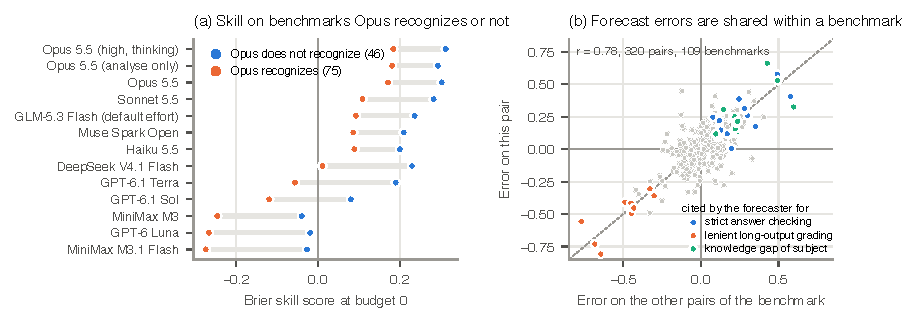
\includegraphics[width=\linewidth]{figures/fig_analysis.pdf}
  \vspace{-9pt}
  \caption{(a) Every forecaster's budget-0 Brier skill score (against always predicting 0.627, on 847 items) is lower on the 75 benchmarks Opus recognizes than on the 46 it does not. Rows without an effort are at low effort, ``analyse only'' is Opus told not to solve the item, and Appendix~\ref{app:judges} describes the models used only here. (b) Each calibration-set pair's forecast error, mean forecast minus success rate, against the mean error of the other pairs on its benchmark. Colors mark benchmarks the forecaster cited when explaining its errors, for illustration only.}
  \label{fig:analysis}
\end{figure}

\subsection{Where Opus's lead comes from}
\label{sec:lead}

Beyond calibration, which the fitted constants remove, Opus's lead lies in ranking items within a pair and in judging a benchmark's overall difficulty, and only the first follows general capability closely. We split each forecaster's budget-0 Brier gap to Opus on the calibration set by successive oracle corrections, recalibrating with its own $a$ and $b$ (calibration), then shifting each benchmark's logits to match its success rate (benchmark level), then each pair's (subject level), and leaving the error within pairs (ranking). Table~\ref{tab:lead} in Appendix~\ref{app:more} gives the parts, and the subject level is negligible.

The ranking loss falls closely with general capability (Appendix~\ref{app:more}). It does not need remembered results, since on the MathArena sets, written after Opus's cutoff, Opus still ranks items better than Sonnet and Haiku.

The benchmark-level loss follows capability only loosely. Sol loses as much there as Haiku, which scores far lower on the index, while Sonnet loses little although it recognizes far fewer benchmarks than Opus (Section~\ref{sec:memory}). Whether this edge comes from knowledge of the benchmarks and their systems or from how these models judge, our data cannot tell.

\subsection{Recognition and accuracy}
\label{sec:memory}

The estimates lean toward an advantage from recognizing a benchmark, but whether recognition helps stays open. The question matters because language models can memorize benchmarks \cite{oren2024contamination}, and a forecaster that remembered published results would offer a lookup rather than a prior. Thirteen forecasters (eleven models, Appendix~\ref{app:judges}) forecast the 847 items of one pair per calibration-set benchmark, and each model is shown three items of each benchmark without its name and asked which benchmark they come from. It recognizes a benchmark when the name it gives matches the benchmark or its source dataset. Opus recognizes 75 of the 121 benchmarks, more than any other model.

A recognition advantage would show as Opus losing less skill than the others on the benchmarks it recognizes. Every forecaster scores lower on these benchmarks (Figure~\ref{fig:analysis}a), so they are harder for all, and Opus loses less than eight of the ten others (average difference in differences $+0.06$, 95\% CI $[-0.04, +0.17]$, Appendix~\ref{app:judges}). Part of this lean comes from miscalibration, since recalibrating the six forecasters with fitted constants lowers every one of their differences. The other forecasters also recognize benchmarks themselves, so they are weaker rather than recognition-free controls.

Opus's thinking summaries at high effort rest mainly on item difficulty, and those that recall published results do not come with a lower Brier (Appendix~\ref{app:judges}).

\subsection{Where the forecast goes wrong}
\label{sec:errors}

The forecast's errors are mostly shared by every subject on a benchmark. On the calibration set, most of the pair-level error lies at the benchmark level (intraclass correlation 0.72), and a pair's error closely tracks the mean error of the other pairs on its benchmark (Figure~\ref{fig:analysis}b). The benchmark component is heavy-tailed (Appendix~\ref{app:more}).

Shown its errors on the 100 calibration-set benchmarks outside every proxy, under anonymous ids, Opus at high effort named the strictness of answer checking (exact match, executed SQL, formal proofs) as the leading cause in each of three runs, followed by lenient grading of long deliverables, events after the subject's training data, low-resource languages and subjective labels. Our prompt asks the forecaster to consider grading strictness, so this may partly echo it, and we did not test these causes. Possible data errors that the forecaster exposed are in Appendix~\ref{app:data}.

\subsection{What the revealed outcomes add}
\label{sec:labels}

Revealed outcomes repair the forecast where it is wrong about a benchmark and add a little noise where it is right (Section~\ref{sec:gain}). A second forecast that reads the revealed items with their outcomes did not help (Appendix~\ref{app:ablations}). BLE's acquisition rule, which reveals a candidate only when its current prediction lies near 0.5 \cite{lewis1994sequential}, gains only slightly over random order (Appendix~\ref{app:ablations}), as expected when random order is a strong baseline for estimating a level \cite{zhang2025fewer}.

\section{Related work}

Our method joins two lines of work, item-level prediction of AI success and language models as sources of priors. Item-level prediction has used item response models and their amortized variants that predict difficulty from content \cite{lord1980irt, rodriguez2021evaluation, truong2025amortized, jiang2026irt} and efficient subset selection \cite{polo2024tiny, zhang2025fewer}. ADeLe predicts success from 18 demand scales annotated by a language model \cite{zhou2026adele}, and the error factors our forecaster names resemble demand scales selected by its own errors. Language models have forecast real-world events \cite{halawi2024forecasting}, supplied priors for statistical models \cite{capstick2024autoelicit} and given cheap predictions that a few labels correct \cite{angelopoulos2023ppi}, and Equation~\eqref{eq:model} is a hierarchical Bayesian version of the last.

\section{Limitations}
\label{sec:limits}

\begin{itemize}
  \item \textbf{Overlap with the calibration set.} The held-out proxies were first evaluated after the forecaster, the prompt, $\sigma_B$ and $\sigma_P$ were fixed, but their 21 benchmarks were also in the pool that fixed the baseline's constants and in the calibration set that fixes the remaining constants. Refitting every forecaster's constants without those benchmarks changes its held-out ALC by at most 0.001 (Appendix~\ref{app:more}).
  \item \textbf{Sample size.} Twenty-seven held-out pairs give intervals of about $\pm 0.016$.
  \item \textbf{New or unfamiliar benchmarks.} Opus removes about half of the base rate's pair-level error on calibration-set benchmarks released before 2025 but only about a quarter on those released since, and after its training cutoff the method only matches the baseline, a check we could run on research-level mathematics alone (Section~\ref{sec:cutoff}). The hidden benchmarks come from 2024 to 2026, and $\tau$, fitted on public benchmarks, may understate how much the forecast's reliability varies on them, so the gain on the hidden test may be smaller.
  \item \textbf{Proprietary forecaster.} The main forecaster is a proprietary model behind an API, so results depend on its version, availability and cost. Three open-weight forecasters recover half to two thirds of its gain.
  \item \textbf{Submitted code.} The submitted predictor re-forecasts the revealed items in batched requests at every call, which differ slightly from the separate forecasts in our tables and which we checked offline at two budgets and live on one formative run (Appendix~\ref{app:repro}).
\end{itemize}

\section*{Reproducibility and disclosure}

The code for every number, table and figure, the submitted predictor, the scripts that rebuild the proxy evaluations from measurement-db, and every forecast we collected are at \url{https://github.com/leeminseung/paiec-lm-prior}. Data, model versions, how each forecast was obtained and the prediction algorithm are in Appendix~\ref{app:repro}.

\bibliographystyle{plainnat}
\bibliography{references}

\appendix

\section{Reproducibility}
\label{app:repro}

\paragraph{Data and settings.} The data are measurement-db at revision 54074453 and, for Section~\ref{sec:cutoff}, five MathArena output sets from August and September 2026 (Hugging Face, CC BY-SA 4.0). The main forecaster is \texttt{claude-opus-5-5} at effort \texttt{low} with the prompts in Appendix~\ref{app:prompts}, and bootstrap intervals use 4{,}000 draws (2{,}000 for Table~\ref{tab:lead}) and seed 0. No model was fine-tuned. Claude Code was used as a coding assistant and helped draft this report.

\paragraph{How forecasts were obtained.} Claude forecasts came mostly from the Claude command-line interface, run with only our system prompt, answer schema and effort, and otherwise from the API. Other models ran through OpenRouter with one pinned provider each (open-weight models in fp8, details in the repository). When the interface returned nothing from the requested model, it answered with an earlier model of the same line, for 0.8\% of Opus's proxy forecasts (5.8\% of the first validation proxy's acquisition candidates) and 1.7\% of its calibration-set forecasts, and we kept those answers. On the first validation proxy, 27 refusals were replaced by Sonnet 5.5 forecasts. Forecasts still missing after one retry fall back to 0.575.

\begin{algorithm}[h]
  \caption{Our predictor}
  \label{alg:predict}
  \begin{algorithmic}[1]
    \Require $\textsc{Forecast}(s, i)$, a language model's success probability for $s$ on $i$, made without outcomes
    \Require $\sigma_B$, $\sigma_P$ and $\tau$, fitted once on the calibration set (Section~\ref{sec:model})
    \Require target subject $s$ and item $i$ on benchmark $B$
    \Require revealed outcomes $R = \{(s', j, y_{s'j})\}$ on $B$, from every subject
    \Statex
    \Phase{Forecast, without outcomes}
      \State $q_{si} \gets \textsc{Forecast}(s, i)$
      \For{each $(s', j) \in R$}
        \State $q_{s'j} \gets \textsc{Forecast}(s', j)$
      \EndFor
    \EndPhase
    \Phase{Update the random effects} \Comment{Eq.~\eqref{eq:model}}
      \State $\theta = (u_B, \beta_B$, and $v_{s'B}$ for every subject $s'$ on $B)$
      \State $(\mu, \Sigma) \gets$ mode and covariance of the Laplace approximation to $p(\theta \mid R)$ \label{alg:update}
    \EndPhase
    \Phase{Predict} \Comment{Eq.~\eqref{eq:pred}}
      \State $\mu_u, \mu_\beta, \mu_v \gets$ the entries of $\mu$ for $u_B$, $\beta_B$ and $v_{sB}$
      \State $m \gets (1 + \mu_\beta)\logit q_{si} + \mu_u + \mu_v$ \Comment{predicted logit}
      \State $\sigma^2 \gets$ variance of $u_B + \beta_B \logit q_{si} + v_{sB}$ under $\Sigma$ \label{alg:var}
      \State \Return $\operatorname{sigmoid}\bigl(m / \sqrt{1 + \pi\sigma^2/8}\bigr)$
    \EndPhase
  \end{algorithmic}
\end{algorithm}

\paragraph{Fitting the random effects.} Line~\ref{alg:update} of Algorithm~\ref{alg:predict} maximizes the log posterior
\begin{equation*}
  \sum_{(s', j) \in R} \log \mathrm{Bernoulli}\bigl(y_{s'j} \mid \operatorname{sigmoid}((1 + \beta_B)\logit q_{s'j} + u_B + v_{s'B})\bigr) - \frac{u_B^2}{2\sigma_B^2} - \frac{\beta_B^2}{2\tau^2} - \sum_{s'} \frac{v_{s'B}^2}{2\sigma_P^2}
\end{equation*}
by Newton steps, halving any step that lowers it, and inverts the negative Hessian at the mode for the Laplace covariance $\Sigma$. Line~\ref{alg:var} takes $\sigma^2 = x^\top \Sigma x$, with $x$ selecting $u_B + \beta_B \logit q_{si} + v_{sB}$.

\paragraph{Submitted code.} When the batched request holding the target fails, the target alone is requested once more. Revealed items still without a forecast are left out of the update, and a target without one falls back to 0.575 with every revealed item entered at that value. Opus refuses some biology items, which then take this path. At budgets 7 and 31 on ten sampled targets per pair of the validation proxies, the batched forecasts correlate at 0.918 with the separate forecasts used in our tables and raise Brier by up to 0.006, about twice what the update gains on the held-out proxies. The submission also completed a live formative run on Codabench.

\section{Prompts}
\label{app:prompts}

Every forecaster gets the same system prompt, given below with its analyse-only variant and the recognition prompt.

\paragraph{Forecaster.} The system prompt follows. The user message is a JSON object with the subject's fields and the item's content (middle-truncated at 12{,}000 characters), features, interactors and anonymous benchmark id. The submission uses the same prompt in a batched form that lists several items of one subject and returns one probability per item, with revealed items truncated at 4{,}000 characters.
\begin{quote}\small
You estimate the probability that a given AI system (the subject) answers a given benchmark item correctly, without running the system.

The subject is described by its model name, provider, release date, access date, harness (the agent scaffold or evaluation runner that drove the model), harness version, reasoning effort and extra settings. The item gives the full task text the subject received, item features, interactors (other tools or agents involved) and an anonymous benchmark id. Empty values mean unknown.

Think about how capable this system is under these settings, how hard this particular item is, and how strictly tasks like this are usually graded. Your answer is scored by Brier score, the squared error between your probability and the 0/1 outcome, so give a calibrated probability.

Answer with JSON: \{"probability": <number from 0 to 1>\}.
\end{quote}

\paragraph{Analyse-only variant.} The same prompt followed by ``Do not try to solve the item or work out its answer yourself. Judge only from the outside: what kind of task it is, what capabilities it needs, how long it is, how strictly tasks like this are usually graded, and how capable this subject is under these settings.''

\paragraph{Recognition.} Three items of one benchmark (the first three of a pair by key, each cut to 1{,}200 characters), with no subject and no name, and the instruction to say whether the model recognizes the benchmark from its training, to give its name and what it recalls about how AI systems score on it, and to prefer ``not recognized'' over a confident wrong name.

\section{Proxy evaluations}
\label{app:proxies}

Each proxy draws recent benchmarks and recent named systems from measurement-db (Table~\ref{tab:proxies}). Candidate pairs use named systems released in 2025 or later by the nine providers the organizers list, benchmarks released in 2024 or later, and 88 to 152 items per pair.

\begin{table}[h]
  \caption{Benchmarks and ALC of each proxy evaluation. Shading compares the Opus forecast and ours with the baseline of the same proxy.}
  \label{tab:proxies}
  \centering
  \small
  \setlength{\tabcolsep}{4pt}
  \begin{tabular}{p{0.12\linewidth}p{0.5\linewidth}ccc}
    \toprule
    Proxy & Benchmarks & Baseline & Forecast & Ours \\
    \midrule
    Validation 1 & BenGER, MedHELM MedCalc, OpenBioRQ, Robust Reasoning, S-GRADES, SWE-rebench, WorkArena & 0.205 & \shd{0.228}{0.205}{0.045}{1} 0.228 & \shd{0.189}{0.205}{0.045}{1} 0.189  \\
    Validation 2 & AlgoTune, AppWorld, BABILong, DAVE, KernelBench, MedHELM MEDEC, WorldCentralBanks & 0.245 & \shd{0.23}{0.245}{0.045}{1} 0.230 & \shd{0.227}{0.245}{0.045}{1} 0.227  \\
    Held-out 1 & REAL, EDU-CIRCUIT-HW, tau2-bench, Software World Models, MathConstraint, Agentic Review Perturbation, SketchJudge & 0.241 & \shd{0.245}{0.241}{0.045}{1} 0.245 & \shd{0.222}{0.241}{0.045}{1} 0.222  \\
    Held-out 2 & MedHELM MedHallu, WorkBench Revisited, MMLU-Pro, MedHELM Medbullets, AGI-Elo, RISEBench, HealthAdminBench & 0.194 & \shd{0.123}{0.194}{0.045}{1} 0.123 & \shd{0.131}{0.194}{0.045}{1} 0.131  \\
    Held-out 3 & Multi-SWE-bench, FaithCoT, VisualWebArena, Legal RAG Bench, HLE, ICPC-2 Code Selector, NatureBench & 0.208 & \shd{0.149}{0.208}{0.045}{1} 0.149 & \shd{0.155}{0.208}{0.045}{1} 0.155  \\
    \bottomrule
  \end{tabular}
\end{table}

\section{Baselines}
\label{app:baselines}

Every baseline predicts from revealed outcomes without a forecast, and only the IRT model also reads subject and item attributes. Let a pair $(s, B)$ have $x$ successes among $k$ revealed outcomes and other subjects on $B$ have $S$ successes among $N$.

\paragraph{Empirical Mean.} $\hat p = x/k$, and 0.5 when $k = 0$ \cite{paiecbaselines2026}. One revealed outcome makes it predict 0 or 1, so it scores worse than answering 0.5.

\paragraph{J2.} A pooled shrinkage rule that a participant published under this name \cite{yamasaki2026j2}, $\hat p = (x + 2c)/(k + 2)$ with $c = (S + 2)/(N + 4)$.

\paragraph{Beta-binomial baseline.} A benchmark-level rate with prior $\mathrm{Beta}(A_0 m, A_0(1-m))$ is updated by the other subjects, and the pair's rate, with a Beta prior of strength $A$ centred on that posterior mean, by its own outcomes,
\begin{equation*}
  \hat p = \frac{x + A\,c}{k + A}, \qquad c = \frac{S + A_0\, m}{N + A_0}.
\end{equation*}
The prior mean $m = 0.575$ and the strength $A = 4$ were fit to minimize ALC by replaying the competition protocol on 40 candidate benchmarks of measurement-db, which is why $m$ differs from the mean pair success rate 0.627 used as the reference in Brier skill scores, and $A_0 = 4$ follows J2.

\paragraph{Outcome-only IRT model.} $\logit \Pr(y_{si} = 1) = \mu + \beta_B + \theta_{sB} + \delta_i$, with a benchmark effect, a subject-within-benchmark effect and an item effect. The subject effect has a prior mean from a ridge regression on provider, release date, reasoning effort and whether a harness is recorded, plus shrunken model-name effects, and the item effect a prior mean from text length, a multiple-choice flag and a code flag. It is fit on 105 measurement-db benchmarks outside the proxies (9{,}047 pairs). Predictions use a Laplace posterior given all revealed outcomes on the benchmark.

\section{Details of the results}
\label{app:more}

\paragraph{Worked example (Section~\ref{sec:infer}).} On tau2-bench Opus's within-pair AUC is 0.69 for GPT-4.1 mini and 0.81 for o4-mini, and its mean forecast of 0.27 becomes 0.30 at budget 0 after the shrinkage of Equation~\eqref{eq:pred}. Outcomes from both subjects raise $u_B$ to $+1.78$ by budget 7. The two pairs gain 0.023 and 0.017 in ALC over the baseline, below the median of 0.036 over the 27 held-out pairs.

\paragraph{Calibration of Opus (Section~\ref{sec:model}).} Fitting $a + b \logit q_{si}$ in place of the offset on the calibration set, with $\sigma_B$ and $\sigma_P$ as in Section~\ref{sec:model} and $a$ and $b$ by maximum likelihood, gives $b = 1.01$ (95\% CI $[0.89, 1.13]$) and $a = -0.11$ ($[-0.32, +0.06]$).

\paragraph{Outcome-only predictors (Section~\ref{sec:results}).} At budget 0 the baseline scores 0.254 and the IRT model 0.247 on the held-out proxies, against 0.250 for answering 0.5.

\paragraph{Per proxy (Section~\ref{sec:gain}).} On the held-out proxies the update adds 0.003 to the forecast alone (95\% CI $[-0.009, +0.021]$). A held-out pair's mean prediction lies on average 0.095 from its success rate at budget 0, against 0.242 for the baseline, 0.113 and 0.117 at budgets 1 and 7, and 0.063 at budget 31, against the baseline's 0.076 (Figure~\ref{fig:main}b). On the validation proxies the forecast alone scores 0.229 against the baseline's 0.225. Across all five proxies the update adds 0.010 of the 0.034. Per proxy (Table~\ref{tab:proxies}), it repairs validation 1 and held-out 1, where the forecast alone loses to the baseline, costs a little on held-out 2 and 3, where the forecast is already good, and helps a little on validation 2.

\paragraph{Other forecasters (Section~\ref{sec:ladder}).} Recalibration alone brings the raw held-out ALC of Sol from 0.254 to 0.192 and of Luna from 0.258 to 0.216, and the update then adds 0.005 to 0.025 for the other forecasters, against 0.003 for Opus. On the calibration set the OpenAI models' mean forecast is 0.66 to 0.73 against a mean item success rate of 0.51, and 38\% of Sol's forecasts are 0.9 or higher, against 11\% of Opus's. Held-out ALC has a rank correlation of $-0.94$ with the capability index across the nine forecasters, and models level on the index score alike (Sonnet and Sol 0.179 and 0.178, Luna and GLM-5.3 Flash 0.191 and 0.192). At low effort the index rates Opus and Sol 35, Terra 29, Sonnet 26 and Haiku 19.

\paragraph{MathArena (Section~\ref{sec:cutoff}).} The three September sets are ArXivMath, BrokenArXiv and ArXivLean, with 19 system--set pairs, and most of their systems were released after the cutoff. Each set has 53 problems with one or two attempts per problem. We reveal 31 problems per pair in random order and score the rest, averaging five random splits, with intervals over pairs. The forecast alone scores 0.266 against 0.195 for the Beta-binomial baseline, with a mean forecast of 0.12 against a mean success rate of 0.49, even when the system is Opus 5.5 itself, and our method scores 0.191. The benchmark-specific slope lowers ALC by 0.004 ($[0.000, 0.007]$) here, against a cost of 0.0006 ($[0.0001, 0.0012]$) on the held-out proxies. On the two August sets (33 pairs), also written after the cutoff and used to design the slope, our method's ALC exceeds the baseline's by 0.008 ($[-0.004, +0.021]$), and by 0.021 ($[+0.006, +0.037]$) without the slope.

\begin{table}[h]
  \caption{Beyond calibration, Opus's lead lies in ranking items within a pair and in judging each benchmark's difficulty. Budget-0 Brier gap to Opus (Brier 0.194) on the calibration set (109 benchmarks with at least two pairs, 2{,}224 items every forecaster answered), split by successive oracle corrections (Section~\ref{sec:lead}, definitions below). Higher is worse.}
  \label{tab:lead}
  \centering
  \small
  \begin{tabular}{lcccccc}
    \toprule
    Forecaster & Total [95\% CI] & Calibration & Benchmark & Subject & Ranking \\
    \midrule
    Sonnet 5.5 & \shq{worse}{0.013}{0.101} $+0.013$ [$+0.006$, $+0.020$] & \shq{worse}{0.002}{0.101} $+0.002$ & \shq{worse}{0.003}{0.101} $+0.003$ & \shq{worse}{0.001}{0.101} $+0.001$ & \shq{worse}{0.006}{0.101} $+0.006$  \\
    Haiku 5.5 & \shq{worse}{0.028}{0.101} $+0.028$ [$+0.016$, $+0.041$] & \shq{worse}{0.006}{0.101} $+0.006$ & \shq{worse}{0.011}{0.101} $+0.011$ & \shq{worse}{0.002}{0.101} $+0.002$ & \shq{worse}{0.009}{0.101} $+0.009$  \\
    GPT-6.1 Sol & \shq{worse}{0.079}{0.101} $+0.079$ [$+0.057$, $+0.102$] & \shq{worse}{0.061}{0.101} $+0.061$ & \shq{worse}{0.011}{0.101} $+0.011$ & \shq{worse}{0.001}{0.101} $+0.001$ & \shq{worse}{0.006}{0.101} $+0.006$  \\
    GPT-6.1 Terra & \shq{worse}{0.054}{0.101} $+0.054$ [$+0.039$, $+0.070$] & \shq{worse}{0.035}{0.101} $+0.035$ & \shq{worse}{0.009}{0.101} $+0.009$ & \shq{worse}{0.002}{0.101} $+0.002$ & \shq{worse}{0.007}{0.101} $+0.007$  \\
    GPT-6 Luna & \shq{worse}{0.101}{0.101} $+0.101$ [$+0.079$, $+0.123$] & \shq{worse}{0.065}{0.101} $+0.065$ & \shq{worse}{0.022}{0.101} $+0.022$ & \shq{worse}{0.003}{0.101} $+0.003$ & \shq{worse}{0.011}{0.101} $+0.011$  \\
    GLM-5.3 & \shq{worse}{0.029}{0.101} $+0.029$ [$+0.019$, $+0.038$] & \shq{worse}{0.005}{0.101} $+0.005$ & \shq{worse}{0.009}{0.101} $+0.009$ & \shq{worse}{0.003}{0.101} $+0.003$ & \shq{worse}{0.012}{0.101} $+0.012$  \\
    GLM-5.3 Flash & \shq{worse}{0.03}{0.101} $+0.030$ [$+0.020$, $+0.041$] & \shq{worse}{0.007}{0.101} $+0.007$ & \shq{worse}{0.011}{0.101} $+0.011$ & \shq{worse}{0.002}{0.101} $+0.002$ & \shq{worse}{0.01}{0.101} $+0.010$  \\
    DeepSeek V4.1 Flash & \shq{worse}{0.037}{0.101} $+0.037$ [$+0.025$, $+0.048$] & \shq{worse}{0.018}{0.101} $+0.018$ & \shq{worse}{0.009}{0.101} $+0.009$ & \shq{worse}{0.002}{0.101} $+0.002$ & \shq{worse}{0.008}{0.101} $+0.008$  \\
    \bottomrule
  \end{tabular}
\end{table}

\paragraph{Gap split (Section~\ref{sec:lead}).} The ranking loss has a rank correlation with the capability index of $-0.92$ across the nine forecasters (95\% CI over benchmarks $[-0.95, -0.61]$), and the benchmark-level loss one of $-0.54$ ($[-0.92, -0.27]$). Sol and Sonnet, level on the index, lose the same 0.006 to ranking (difference $-0.001$, $[-0.004, +0.003]$). On MathArena, Opus's within-pair AUC is 0.61 against 0.54 for Sonnet and 0.51 for Haiku, differences whose intervals exclude zero but are optimistic, since the pairs of a set share problems, and Opus orders the systems no better than they do (pair-level correlation 0.37 against 0.51 and 0.57). At the benchmark level Sol loses 0.011, 0.008 more than Sonnet ($[+0.001, +0.016]$, not significant after correcting for the four pairwise comparisons we ran). Across benchmarks, the rank correlation between the mean forecast and the observed success rate is 0.70 for Opus and 0.65 for Sonnet, against 0.44 to 0.61 for the others.

\paragraph{Shared errors (Section~\ref{sec:errors}).} The intraclass correlation of the pair-level error within benchmarks is 0.72 (95\% CI $[0.56, 0.81]$, 109 benchmarks with at least two pairs), and a pair's error correlates at 0.78 with the mean error of the other pairs on its benchmark. A Student-$t$ with three degrees of freedom fits the 121 benchmark mean errors far better than a normal (log-likelihood $-162$ against $-197$).

\paragraph{Overlap and recent benchmarks (Section~\ref{sec:limits}).} The calibration set also contains 6 of the 27 held-out pairs, with 67 of their 1{,}504 scored items. Opus removes 51\% (95\% CI $[40\%, 61\%]$) of the base rate's mean absolute pair-level error on the 56 calibration-set benchmarks released before 2025 and 28\% ($[4\%, 46\%]$) on the 53 released since (12 have no date). It recognizes 46 of the older benchmarks and 21 of the recent ones, so date and recognition cannot be separated here.

\section{Comparison with the BLE agent}
\label{app:ble}

BLE searches measurement-db for up to five turns, and we gave it a corpus that excludes every proxy benchmark (Table~\ref{tab:ble}). At budget 7 its Brier is lower than ours by 0.007 ($[-0.026, +0.015]$), and its higher AUC may come from reading the revealed items with their outcomes. The sample is not typical, since our update gains 0.005 on it at budget 7 but nothing on all held-out targets (0.174 against 0.172 for the forecast alone). BLE failed on 11 of 270 predictions at budget 0, mostly because Opus 5.5 does not support its forced final tool call. Our budget-7 cost is a range because each stateless submission call re-forecasts the pair's revealed items in one batched request (Section~\ref{sec:method}). The range is that request's mean cost on the validation proxies and leaves out the requests for other subjects' items.

\begin{table}[h]
  \caption{BLE matches our Brier and ranks items better, at up to ten times our cost. Opus 5.5 as the forecaster for both, on ten targets per held-out pair, items both answered. Brier is over all responses, pairs weighted equally, and cost is API spend per prediction. Shading compares with ours. $^{*}$See the text.}
  \label{tab:ble}
  \centering
  \small
  \begin{tabular}{lcccccc}
    \toprule
     & \multicolumn{3}{c}{Budget 0 (259 items)} & \multicolumn{3}{c}{Budget 7 (258 items)} \\
    \cmidrule(lr){2-4}\cmidrule(lr){5-7}
    Predictor & Cost & Brier & AUC & Cost & Brier & AUC \\
    \midrule
    Opus forecast, no update & \$0.010 & \shd{0.168}{0.169}{0.045}{1} 0.168 & \shd{0.717}{0.717}{0.1}{-1} 0.717 & \$0.010 & \shd{0.167}{0.161}{0.045}{1} 0.167 & \shd{0.723}{0.723}{0.1}{-1} 0.723  \\
    Ours & \$0.010 & \shd{0.169}{0.169}{0.045}{1} 0.169 & \shd{0.717}{0.717}{0.1}{-1} 0.717 & \$0.05--0.08$^{*}$ & \shd{0.161}{0.161}{0.045}{1} 0.161 & \shd{0.723}{0.723}{0.1}{-1} 0.723  \\
    BLE agent & \$0.099 & \shd{0.166}{0.169}{0.045}{1} 0.166 & \shd{0.752}{0.717}{0.1}{-1} 0.752 & \$0.079 & \shd{0.155}{0.161}{0.045}{1} 0.155 & \shd{0.792}{0.723}{0.1}{-1} 0.792  \\
    \bottomrule
  \end{tabular}
\end{table}

\section{Variants}
\label{app:ablations}

\begin{table}[h]
  \caption{Apart from dropping the update, no variant changes ALC by more than 0.003. Differences are from our method, and shading compares each ALC with ours in the same block.}
  \label{tab:ablations}
  \centering
  \footnotesize
  \begin{tabular}{lcc}
    \toprule
    \multicolumn{3}{l}{\emph{All five proxies and the three held-out ones, ALC}} \\
    Variant & Five & Held-out \\
    \midrule
    Ours & \shd{0.1846}{0.1846}{0.045}{1} 0.1846 & \shd{0.1692}{0.1692}{0.045}{1} 0.1692  \\
    Without the benchmark-specific slope ($\tau = 0$) & \shd{0.1843}{0.1846}{0.045}{1} 0.1843 & \shd{0.1686}{0.1692}{0.045}{1} 0.1686  \\
    Each pair fitted on its own outcomes only & \shd{0.1856}{0.1846}{0.045}{1} 0.1856 & \shd{0.1711}{0.1692}{0.045}{1} 0.1711  \\
    Opus forecast, no update & \shd{0.1947}{0.1846}{0.045}{1} 0.1947 & \shd{0.1722}{0.1692}{0.045}{1} 0.1722  \\
    IRT model, all features & \shd{0.2183}{0.1846}{0.045}{1} 0.2183 &  \\
    \quad without model-identity effects & \shd{0.2178}{0.1846}{0.045}{1} 0.2178 &  \\
    \quad without subject features & \shd{0.2185}{0.1846}{0.045}{1} 0.2185 &  \\
    \quad without item features & \shd{0.2186}{0.1846}{0.045}{1} 0.2186 &  \\
    \midrule
    \multicolumn{3}{l}{\emph{Validation proxies, ALC (ours 0.2078)}} \\
    Variant & ALC & $\Delta$ [95\% CI] \\
    \midrule
    Without the benchmark-specific slope ($\tau = 0$) & \shd{0.2079}{0.2078}{0.045}{1} 0.2079 & $+0.000$ [$-0.001$, $+0.001$]  \\
    Opus at medium instead of low effort & \shd{0.2062}{0.2078}{0.045}{1} 0.2062 & $-0.002$ [$-0.005$, $+0.002$]  \\
    Student-$t$ prior on $u_B$ (3 degrees of freedom, scale 0.58) & \shd{0.2086}{0.2078}{0.045}{1} 0.2086 & $+0.001$ [$-0.006$, $+0.008$]  \\
    Forecast that reads revealed outcomes, at budgets 1--7 & \shd{0.2098}{0.2078}{0.045}{1} 0.2098 & $+0.002$ [$-0.005$, $+0.010$]  \\
    \quad averaged with ours on the logit scale & \shd{0.2063}{0.2078}{0.045}{1} 0.2063 & $-0.002$ [$-0.005$, $+0.002$]  \\
    \midrule
    \multicolumn{3}{l}{\emph{Acquisition, all five proxies, ALC (random order 0.1846)}} \\
    BLE acquisition rule & \shd{0.182}{0.1846}{0.045}{1} 0.1820 & $-0.003$ [$-0.005$, $-0.0002$]  \\
    \bottomrule
  \end{tabular}
\end{table}

Higher effort leaves every forecaster we reran where it was (Table~\ref{tab:effort}). Opus at medium effort is in Table~\ref{tab:ablations}. Sonnet and Haiku at medium effort produce about as many output tokens as at low effort on these items (median 231 against 237 for Sonnet). GPT-6.1 Sol at high effort produces about seven times as many (mean 774 against 114 on 30 items), yet its forecasts correlate at 0.96 with those at low effort and stay as optimistic (mean 0.73 against a success rate of 0.50 on these items).

\begin{table}[h]
  \caption{Higher effort leaves every forecaster within its 95\% interval of low effort. Skill and AUC are budget-0 values on the 847-item subset (Appendix~\ref{app:judges}), on the items both runs answered, with intervals over its 121 pairs. ALC is on the three held-out proxies with each run's own constants.}
  \label{tab:effort}
  \centering
  \small
  \begin{tabular}{llccc}
    \toprule
    Forecaster & Measure & Low & Higher effort & Difference [95\% CI] \\
    \midrule
    Opus 5.5, high & Skill & 0.224 & 0.234 & \shd{0.01}{0.0}{0.05}{-1} $+0.010$ [$-0.005$, $+0.026$]  \\
     & AUC & 0.689 & 0.712 & \shd{0.023}{0.0}{0.05}{-1} $+0.023$ [$-0.013$, $+0.065$]  \\
    Sonnet 5.5, medium & Skill & 0.178 & 0.175 & \shd{-0.003}{0.0}{0.05}{-1} $-0.003$ [$-0.016$, $+0.009$]  \\
     & AUC & 0.653 & 0.665 & \shd{0.012}{0.0}{0.05}{-1} $+0.012$ [$-0.021$, $+0.046$]  \\
    Haiku 5.5, medium & Skill & 0.134 & 0.134 & \shd{0.0}{0.0}{0.05}{-1} $+0.000$ [$-0.026$, $+0.024$]  \\
     & AUC & 0.634 & 0.619 & \shd{-0.015}{0.0}{0.05}{-1} $-0.015$ [$-0.051$, $+0.022$]  \\
    GPT-6.1 Sol, high & Skill & $-0.039$ & $-0.040$ & \shd{-0.0}{0.0}{0.05}{-1} $-0.000$ [$-0.025$, $+0.025$]  \\
     & AUC & 0.685 & 0.679 & \shd{-0.006}{0.0}{0.05}{-1} $-0.006$ [$-0.044$, $+0.031$]  \\
    GLM-5.3, high & ALC & 0.187 & 0.190 & \shd{0.003}{0.0}{0.05}{1} $+0.003$ [$-0.002$, $+0.009$]  \\
    GLM-5.3 Flash, high & ALC & 0.192 & 0.189 & \shd{-0.003}{0.0}{0.05}{1} $-0.003$ [$-0.008$, $+0.003$]  \\
    \bottomrule
  \end{tabular}
\end{table}


\section{Forecasters on the 847-item subset}
\label{app:judges}

The thirteen forecasters are the rows of Table~\ref{tab:judges}, eleven models with Opus 5.5 in three setups (low effort, low effort told not to solve the item, and high effort with its thinking summaries returned). GLM-5.3 joined later and is not in this comparison. A second model (Haiku 5.5) checks each recognition answer against the benchmark's entry in the measurement-db catalog. Opus recognizes 57 benchmarks by name and 18 by source dataset. On the benchmarks Opus recognizes, Opus at low effort loses 0.13 in Brier skill score, against 0.11 to 0.25 for the ten other forecasters. The average difference in differences, $+0.06$, exceeds Opus's margin of 0.05 over Sonnet on these items. Recalibration lowers the OpenAI models' differences in differences by about half, to $+0.04$ to $+0.05$.

\begin{table}[h]
  \caption{Thirteen forecasters at budget 0 on 847 items (121 benchmarks). BSS is the Brier skill score against always predicting 0.627, the mean pair success rate of measurement-db, a reference that needs no outcome from the scored items. Named counts benchmarks whose name or source dataset the model gave correctly (MiniMax M3 answered for 86 benchmarks). The last column is Opus (low)'s BSS gap between named and other benchmarks minus the same gap for that forecaster, positive when it favors a recognition advantage.}
  \label{tab:judges}
  \centering
  \footnotesize
  \setlength{\tabcolsep}{2.6pt}
  \begin{tabular}{lccccccc}
    \toprule
    Forecaster & Brier & BSS & AUC & Named & \multicolumn{2}{c}{BSS on Opus-named / not} & Difference in differences \\
    \midrule
    Opus 5.5, high, thinking & 0.203 & \shd{0.234}{0.0}{0.234}{-1} 0.234 & \shs{better}{0.712}{0.58}{0.72} 0.712 & \shs{neutral}{75.0}{0}{75} 75 & \shd{0.184}{0.0}{0.312}{-1} 0.184 & \shd{0.312}{0.0}{0.312}{-1} 0.312 &  \\
    Opus 5.5, low, analyse only & 0.206 & \shd{0.226}{0.0}{0.234}{-1} 0.226 & \shs{better}{0.698}{0.58}{0.72} 0.698 & \shs{neutral}{75.0}{0}{75} 75 & \shd{0.181}{0.0}{0.312}{-1} 0.181 & \shd{0.293}{0.0}{0.312}{-1} 0.293 &  \\
    Opus 5.5, low & 0.206 & \shd{0.224}{0.0}{0.234}{-1} 0.224 & \shs{better}{0.686}{0.58}{0.72} 0.686 & \shs{neutral}{75.0}{0}{75} 75 & \shd{0.172}{0.0}{0.312}{-1} 0.172 & \shd{0.302}{0.0}{0.312}{-1} 0.302 &  \\
    Sonnet 5.5, low & 0.218 & \shd{0.178}{0.0}{0.234}{-1} 0.178 & \shs{better}{0.653}{0.58}{0.72} 0.653 & \shs{neutral}{30.0}{0}{75} 30 & \shd{0.109}{0.0}{0.312}{-1} 0.109 & \shd{0.283}{0.0}{0.312}{-1} 0.283 & $+0.043$ [$-0.041$, $+0.123$]  \\
    GLM-5.3 Flash, default effort & 0.225 & \shd{0.15}{0.0}{0.234}{-1} 0.150 & \shs{better}{0.654}{0.58}{0.72} 0.654 & \shs{neutral}{31.0}{0}{75} 31 & \shd{0.093}{0.0}{0.312}{-1} 0.093 & \shd{0.236}{0.0}{0.312}{-1} 0.236 & $+0.012$ [$-0.118$, $+0.131$]  \\
    Muse Spark Open & 0.230 & \shd{0.136}{0.0}{0.234}{-1} 0.136 & \shs{better}{0.643}{0.58}{0.72} 0.643 & \shs{neutral}{18.0}{0}{75} 18 & \shd{0.087}{0.0}{0.312}{-1} 0.087 & \shd{0.21}{0.0}{0.312}{-1} 0.210 & $-0.008$ [$-0.113$, $+0.106$]  \\
    Haiku 5.5, low & 0.230 & \shd{0.134}{0.0}{0.234}{-1} 0.134 & \shs{better}{0.634}{0.58}{0.72} 0.634 & \shs{neutral}{26.0}{0}{75} 26 & \shd{0.089}{0.0}{0.312}{-1} 0.089 & \shd{0.2}{0.0}{0.312}{-1} 0.200 & $-0.020$ [$-0.143$, $+0.097$]  \\
    DeepSeek V4.1 Flash, low & 0.239 & \shd{0.098}{0.0}{0.234}{-1} 0.098 & \shs{better}{0.648}{0.58}{0.72} 0.648 & \shs{neutral}{42.0}{0}{75} 42 & \shd{0.012}{0.0}{0.312}{-1} 0.012 & \shd{0.23}{0.0}{0.312}{-1} 0.230 & $+0.088$ [$-0.028$, $+0.212$]  \\
    GPT-6.1 Terra, low & 0.254 & \shd{0.042}{0.0}{0.234}{-1} 0.042 & \shs{better}{0.655}{0.58}{0.72} 0.655 & \shs{neutral}{37}{0}{75} 37 & \shd{-0.056}{0.0}{0.312}{-1} $-0.056$ & \shd{0.19}{0.0}{0.312}{-1} 0.190 & $+0.115$ [$-0.021$, $+0.254$]  \\
    GPT-6.1 Sol, low & 0.276 & \shd{-0.039}{0.0}{0.234}{-1} $-0.039$ & \shs{better}{0.683}{0.58}{0.72} 0.683 & \shs{neutral}{47}{0}{75} 47 & \shd{-0.119}{0.0}{0.312}{-1} $-0.119$ & \shd{0.081}{0.0}{0.312}{-1} 0.081 & $+0.069$ [$-0.111$, $+0.247$]  \\
    GPT-6 Luna, low & 0.310 & \shd{-0.167}{0.0}{0.234}{-1} $-0.167$ & \shs{better}{0.605}{0.58}{0.72} 0.605 & \shs{neutral}{24}{0}{75} 24 & \shd{-0.266}{0.0}{0.312}{-1} $-0.266$ & \shd{-0.019}{0.0}{0.312}{-1} $-0.019$ & $+0.117$ [$-0.062$, $+0.307$]  \\
    MiniMax M3.1 Flash & 0.312 & \shd{-0.175}{0.0}{0.234}{-1} $-0.175$ & \shs{better}{0.622}{0.58}{0.72} 0.622 & \shs{neutral}{28.0}{0}{75} 28 & \shd{-0.274}{0.0}{0.312}{-1} $-0.274$ & \shd{-0.026}{0.0}{0.312}{-1} $-0.026$ & $+0.117$ [$-0.075$, $+0.320$]  \\
    MiniMax M3 & 0.308 & \shd{-0.163}{0.0}{0.234}{-1} $-0.163$ & \shs{better}{0.591}{0.58}{0.72} 0.591 & \shs{neutral}{30.0}{0}{75} 30 & \shd{-0.245}{0.0}{0.312}{-1} $-0.245$ & \shd{-0.039}{0.0}{0.312}{-1} $-0.039$ & $+0.076$ [$-0.126$, $+0.276$]  \\
    \bottomrule
  \end{tabular}
\end{table}

\paragraph{Name matches only.} Counting name matches only (57 benchmarks), the average is $+0.05$ ($[-0.06, +0.15]$), favoring Opus for seven of the ten.

\paragraph{Stated reasoning.} The forecaster's stated reasoning rests mainly on item difficulty. Opus at high effort returned thinking summaries for 826 items, 744 of them with reasoning, and Sonnet 5.5 labeled what each summary relies on from the summary alone. Item difficulty is the main basis for 56\% of all 826 summaries. Of the 744 summaries with reasoning, 88\% discuss item difficulty, 55\% the subject's capability, 48\% name the benchmark, 37\% grading and 28\% recall published results. Items whose summary names the benchmark are predicted no better than the rest (Brier 0.221 against 0.205). Items whose summary recalls published results are predicted about as well as the rest (Brier 0.211 against 0.214) but are forecast closer to their pair's success rate (mean absolute difference 0.164 against 0.187), which is where remembered results would act.

\paragraph{Analyse-only instruction.} Telling the forecaster not to solve the item changes its forecasts little (correlation 0.976, Brier 0.207 against 0.206 on the 844 items both answered).

\section{Possible data errors found by the forecaster}
\label{app:data}

Items that the forecaster rated at 0.85 or higher but that at most 15\% of at least five subjects solved point to possible errors in the public data. In RealTimeQA the answer index is stored as the string ``0'' and grading compares predictions by native equality, so integer answers may always be marked wrong. Of its 7{,}877 items, 39\% are solved by no subject and only 3\% by 90\% or more, low for multiple-choice news questions, although the answer keys we checked are correct. In CMMLU, a chemistry item failed by all six subjects has a correct key, but the grading pattern accepts only an ASCII colon after the answer prefix. In the other direction, MorphKV items rated below 0.15 are solved by every subject, which suggests more lenient grading than the item text implies. These are candidates for the maintainers to check, in the spirit of \citet{truong2025bugs}.

\end{document}
